\begin{abstract}
Existing regression models tend to fall short in both accuracy and uncertainty estimation when the label distribution is imbalanced. In this paper, we 
propose a probabilistic deep learning model, dubbed variational imbalanced regression (VIR), which not only performs well in imbalanced regression but naturally produces reasonable uncertainty estimation as a byproduct. 
Different from typical variational autoencoders assuming I.I.D. representations (a data point's representation is not directly affected by other data points), our VIR borrows data with similar regression labels to compute the latent representation's variational distribution; furthermore, different from deterministic regression models producing point estimates, VIR predicts the entire normal-inverse-gamma distributions and modulates the associated conjugate distributions to impose probabilistic reweighting on the imbalanced data, thereby providing better uncertainty estimation. Experiments in several real-world datasets show that our VIR can outperform state-of-the-art imbalanced regression models in terms of both accuracy and uncertainty estimation. Code will soon be available at \url{https://github.com/Wang-ML-Lab/variational-imbalanced-regression}.
\end{abstract}

\section{Introduction}\label{sec:intro}
Deep regression models are currently the state of the art in making predictions in a continuous label space and have a wide range of successful applications in computer vision~\citep{ExampleCV}, natural language processing~\citep{ExampleNLP}, healthcare~\citep{BIN,CounTS}, recommender systems~\citep{ExposureBias,REN}, etc. 
However, these models fail however when the label distribution in training data is imbalanced. For example, in visual age estimation~\citep{AGEDB}, where a model infers the age of a person given her visual appearance, models are typically trained on imbalanced datasets with overwhelmingly more images of younger adults, leading to poor regression accuracy for images of children or elderly people~\citep{MDLT,DIR}. 
Such unreliability in imbalanced regression settings motivates the need for both \emph{improving performance for the minority} in the presence of imbalanced data and, more importantly, \emph{providing reasonable uncertainty estimation} to inform practitioners on how reliable the predictions are (especially for the minority where accuracy is lower).

Existing methods for deep imbalanced regression (DIR) only focus on improving the accuracy of deep regression models by smoothing the label distribution and reweighting data with different labels~\citep{MDLT,DIR}. On the other hand, methods that provide uncertainty estimation for deep regression models operates under the balance-data assumption and therefore do not work well in the {imbalanced setting~\citep{DER,natPN,TFuncertainty}.}

{
To simultaneously cover these two desiderata, we propose a probabilistic deep imbalanced regression model, dubbed variational imbalanced regression (VIR). 
% VIR is particularly useful for minority data as it can borrow representations from data with similar labels (and naturally weigh them using our probabilistic model) to counteract data sparsity. 
Different from typical variational autoencoders assuming I.I.D. representations (a data point's representation is not directly affected by other data points), {our VIR assumes Neighboring and Identically Distributed (N.I.D.) and borrows data with similar regression labels to compute the latent representation's variational distribution.} Specifically, VIR first encodes a data point into a probabilistic representation and then mix it with neighboring representations (i.e., representations from data with similar regression labels) to produce its final probabilistic representation; 
VIR is therefore particularly useful for minority data as it can borrow probabilistic representations from data with similar labels (and naturally weigh them using our probabilistic model) to counteract data sparsity. 
Furthermore, different from deterministic regression models producing point estimates, VIR predicts the entire Normal Inverse Gamma (NIG) distributions and modulates the associated conjugate distributions by the importance weight computed from the smoothed label distribution to impose probabilistic reweighting on the imbalanced data. This allows the negative log likelihood to naturally put more focus on the minority data, thereby balancing the accuracy for data with different regression labels. Our VIR framework is compatible with any deep regression models and can be trained end to end.} 

% {
% To simultaneously cover these two desiderata, we propose a probabilistic deep imbalanced regression model, dubbed variational imbalanced regression (VIR). VIR is particularly useful for minority data as it can borrow representations from data with similar labels (and naturally weigh them using our probabilistic model) to counteract data sparsity. Different from typical variational autoencoders assuming I.I.D. representation (a data point's representation is not directly affected by other data points), our VIR borrows data with similar regression labels to compute the latent representation's variational distribution. Specifically, VIR first encodes a data point into a probabilistic representation and then mix it with neighboring representations (i.e., representations from data with similar regression labels) to produce its final probabilistic representation. Furthermore, different from deterministic regression models producing point estimates, VIR predicts the entire normal-inverse-gamma distributions and modulates the associated conjugate distributions by the importance weight computed from the smoothed label distribution to impose probabilistic reweighting on the imbalanced data. This allows the negative log likelihood to naturally put more focus on the minority data, thereby balancing the accuracy for data with different regression labels. Our VIR framework is compatible with any deep regression models and can be trained end to end.} 

% \blue{While previous work has studied imbalanced regression and uncertainty estimation \emph{separately}, none of them has considered uncertainty estimation in the imbalanced setting.}

We summarize our contributions as below:
\begin{compactitem}
\item We identify the problem of probabilistic deep imbalanced regression as well as two desiderata, balanced accuracy and uncertainty estimation, for the problem.
\item We propose VIR to simultaneously cover these two desiderata and achieve state-of-the-art performance compared to existing methods.
\item As a byproduct, we also provide strong baselines for benchmarking {high-quality uncertainty estimation and promising prediction performance on imbalanced datasets.}
\end{compactitem}

\section{Related Work}
%
\begin{wrapfigure}{t}{0.6\textwidth}
\centering
\vskip -0.23in
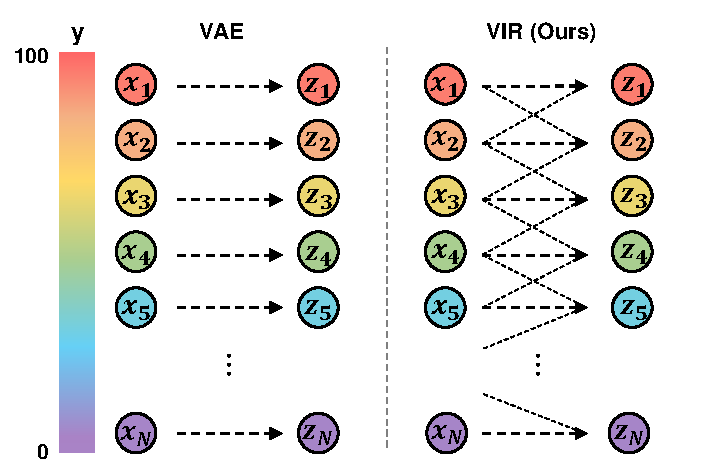
\includegraphics[width=0.6\textwidth]{VIR_1.pdf}
\vskip -0.3cm
    \caption{Comparing inference networks of typical VAE~\citep{VAE} and our VIR. In VAE (\textbf{left}), a data point’s latent representation (i.e., $\z$) is affected only by itself, while in VIR (\textbf{right}), neighbors participate to modulate the final representation.}    
\vskip -0.7cm
\label{encoder-diff}
\end{wrapfigure}
%
\textbf{Variational Autoencoder.} 
Variational autoencoder (VAE)~\citep{VAE} is an unsupervised learning model that aims to infer probabilistic representations from data. However, as shown in Figure~\ref{encoder-diff}, VAE typically assumes I.I.D. representations, where a data point's representation is not directly affected by other data points. In contrast, our VIR borrows data with similar regression labels to compute the latent representation's variational distribution.


\textbf{Imbalanced Regression.} 
Imbalanced regression is under-explored in the machine learning community. Most existing methods for imbalanced regression are direct extensions of the SMOTE algorithm~\citep{SMOTE}, a commonly used algorithm for imbalanced classification, where data from the minority classes is over-sampled. These algorithms usually synthesize augmented data for the minority regression labels by either interpolating both inputs and labels~\citep{IRrelated1} or adding Gaussian noise~\citep{IRrelated2,IRrelated3} (more discussion on augmentation-based methods in the Appendix).

Such algorithms fail to measure the distance in continuous label space and fall short in handling high-dimensional data (e.g., images and text). Recently, DIR~\citep{DIR} addresses these issues by applying kernel density estimation to smooth and reweight data on the continuous label distribution, achieving state-of-the-art performance. However, DIR only focuses on improving the accuracy, especially for the data with minority labels, and therefore does not provide uncertainty estimation, which is crucial to assess the predictions' reliability. \cite{balancedMSE} focuses on re-balancing the mean squared error (MSE) loss for imbalanced regression, and \cite{RankSim} introduces ranking similarity for improving deep imbalanced regression. {In contrast, our VIR provides a principled probabilistic approach to simultaneously achieve these two desiderata, not only improving upon DIR in terms of performance but also producing reasonable uncertainty estimation as a much-needed byproduct to assess model reliability.} There is also related work on imbalanced classification~\citep{Long-Tailed-Age-Classification}, which is related to our work but focusing on classification rather than regression.

\textbf{Uncertainty Estimation in Regression.}
{There has been renewed interest in uncertainty estimation in the context of deep regression models~\citep{DER,uncertain6,uncertain9,kendall2017uncertainties,kuleshov2018accurate,TFuncertainty,uncertain8,song2019distribution,uncertain7,zelikman2020crude}.} Most existing methods directly predict the variance of the output distribution as the estimated uncertainty~\citep{DER,kendall2017uncertainties,zhang2019reducing}, rely on post-hoc confidence interval calibration~\citep{kuleshov2018accurate,song2019distribution,zelikman2020crude}, or using Bayesian neural networks~\citep{NPN,BDL,BDLSurvey}; there are also training-free approaches, such as Infer Noise and Infer Dropout~\citep{TFuncertainty}, which produce multiple predictions from different perturbed neurons and compute their variance as uncertainty estimation. Closest to our work is Deep Evidential Regression (DER)~\citep{DER}, which attempts to estimate both aleatoric and epistemic uncertainty~\citep{Uncertainty4ML,kendall2017uncertainties} on regression tasks by training the neural networks to directly infer the parameters of the evidential distribution, thereby producing uncertainty measures. DER~\citep{DER} is designed for the data-rich regime and therefore fails to reasonably estimate the uncertainty if the data is imbalanced; for data with minority labels, DER~\citep{DER} tends produce unstable distribution parameters, leading to poor uncertainty estimation (as shown in~\secref{sec:exp}).  In contrast, our proposed VIR explicitly handles data imbalance in the continuous label space to avoid such instability; VIR does so by modulating both the representations and the output conjugate distribution parameters according to the imbalanced label distribution, allowing training/inference to proceed as if the data is balance and leading to better performance as well as uncertainty estimation (as shown in~\secref{sec:exp}).

\section{Method}
{In this section we introduce the notation and problem setting, %problem setting, 
provide an overview of our VIR, and then describe details on each of VIR's key components.} 

\subsection{Notation and Problem Setting}\label{sec:problem}
Assuming an imbalanced dataset in continuous space $\{\x_i, y_i \}^{N}_{i=1}$ where $N$ is the total number of data points, $\x_i \in \mathbb{R}^{d}$ is the input, and $y_i\in \mathcal{Y} \subset \mathbb{R} $ is the corresponding label from a continuous label space $\mathcal{Y}$. In practice, $\mathcal{Y}$ is partitioned into B equal-interval bins $[y^{(0)}, y^{(1)}), [y^{(1)}, y^{(2)}), ..., [y^{(B-1)}, y^{(B)})$, with slight notation overload. To directly compare with baselines, we use the same grouping index for target value $b \in \mathcal{B}$ as in~\citep{DIR}. 
%
\begin{wrapfigure}{t}{0.5\textwidth}
\centering
\vskip -0.18in
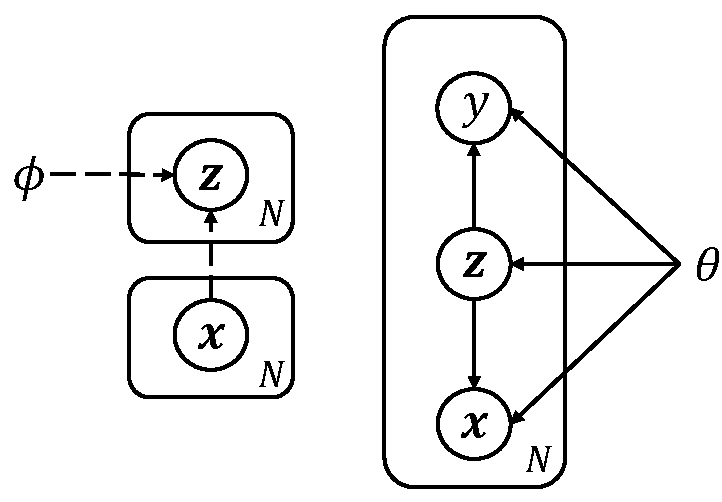
\includegraphics[width=0.38\textwidth]{VIR_2.pdf}
\vskip -0.3cm
    \caption{Overview of our VIR method. \textbf{Left:} The inference model infers the latent representations given input $\x$'s in the neighborhood. \textbf{Right:} The generative model reconstructs the input and predicts the label distribution (including the associated uncertainty) given the latent representation.}
\vskip -1.2cm
\label{vir}
\end{wrapfigure}
%
% We denote representations as $\z_i$, and use $ (\Tilde{\z}_i^{\mu}, \Tilde{\z}_i^{\Sigma}) = q_{\phi}(\z|\x_i; \theta)$ to denote the probabilistic representations for input $\x_i$ generated by a probabilistic encoder parameterized by $\theta$. 
We denote representations as $\z_i$, and use $ (\Tilde{\z}_i^{\mu}, \Tilde{\z}_i^{\Sigma}) = q_{\phi}(\z|\x_i)$ to denote the probabilistic representations for input $\x_i$ generated by a probabilistic encoder parameterized by $\phi$; furthermore, we denote $\Bar{\z}$ as the mean of representation $\z_i$ in each bin, i.e., $\bar{\z} = \frac{1}{N_b} \sum^{N_b}_{i=1} \z_i$ for a bin with $N_b$ data points. 
{Similarly we use $ (\hat{y}_i,\hat{s}_i)$ to denote the mean and variance of the predictive distribution generated by a probabilistic predictor $p_{\theta}(y_i|\z)$.} 

\subsection{Method Overview}
In order to achieve both desiderata in probabilistic deep imbalanced regression (i.e., performance improvement and uncertainty estimation), our proposed variational imbalanced regression (VIR)  operates on both the encoder $q_{\phi}(\z_i|\{\x_i\}^{N}_{i=1})$ and the predictor $p_{\theta}(y_i|\z_i)$.

Typical VAE~\citep{VAE} lower-bounds input $\x_i$'s marginal likelihood; in contrast, VIR lower-bounds the marginal likelihood of input $\x_i$ and labels $y_i$: 
% {
%
% \begin{align*}
% \log p_{\theta}(\{x^{(i)}, y^{(i)}\}^{N}_{i=1}) = \sum^{N}_{i=1} \log p_{\theta}(x^{(i)}, y^{(i)}) = \mathcal{D}_{\mathcal{KL}}(q_{\phi}(z|x^{(i)})||p_{\theta}(z|x^{(i)})) + \mathcal{L}(\theta, \phi; x^{(i)}).
% \end{align*}
\begin{align*}
\log p_{\theta}(\x_i, y_i) = 
 \mathcal{D}_{\mathcal{KL}}\big(q_{\phi}(\z_i|\{\x_i\}^{N}_{i=1})||p_{\theta}(\z_i|\x_i,y_i)\big) + \mathcal{L}(\theta, \phi; \x_i, y_i).
\end{align*}
% }
Note that our variational distribution $q_{\phi}(\z_i|\{\x_i\}^{N}_{i=1})$ (1) does not condition on labels $y_i$, since the task is to predict $y_i$ and (2) conditions on all (neighboring) inputs $\{\x_i\}^{N}_{i=1}$ rather than just $\x_i$. 
%
The second term $\mathcal{L}(\theta, \phi; \x_i, y_i)$ is VIR's evidence lower bound (ELBO), which is defined as: 
%
\begingroup\makeatletter\def\f@size{9}\check@mathfonts
\def\maketag@@@#1{\hbox{\m@th\normalsize\normalfont#1}}%
\begin{align}
\mathcal{L}(\theta, \phi; \x_i, y_i) =   \underbrace{\mathbb{E}_{q} \big[\log p_{\theta}(\x_i|\z_i)\big]}_{\LM_i^{\DM}} +  \underbrace{\mathbb{E}_{q} \big[\log p_{\theta}(y_i|\z_i) \big]}_{\LM_i^{\PM}}
 - \underbrace{\mathcal{D}_{\mathcal{KL}}(q_{\phi}(\z_i|\{\x_i\}^{N}_{i=1})||p_{\theta}(\z_i))}_{\LM_i^{\KM\LM}}. \label{eq:elbo}
\end{align}
\endgroup
%
where {the $p_{\theta}(\z_i)$ is the standard Gaussian prior $\NM(\0,\I)$, following typical VAE~\citep{VAE},} and the expectation is taken over $q_{\phi}(\z_i|\{\x_i\}^{N}_{i=1})$, which infers $\z_i$ by borrowing data with similar regression labels to produce the balanced probabilistic representations, which is beneficial especially for the minority (see~\secref{sec:PRM} for details). 

Different from typical regression models which produce only point estimates for $y_i$, our VIR's predictor, $p_{\theta}(y_i|\z_i)$, directly produces the parameters of the entire NIG distribution for $y_i$ and further imposes probabilistic reweighting on the imbalanced data, thereby producing balanced predictive distributions (more details in~\secref{sec:CDM}). 

% We also add the reconstructor of typical VAE~\citep{VAE} to stabilize the latent variables. In the following, we introduce the details for constructing each of them. Formally, for each datapoint, we have
% %
% \begin{align*}
% q_{\phi}(z|x^{(i)}) &= \mathcal{H} (\mathcal{F} (x_i)) \\
% p_{\theta}(y^{(i)}|z) &= \mathcal{G} (z_i) \\
% p_{\theta}(x^{(i)}|z) &= \mathcal{R} (z_i)
% \end{align*}
% %
% where in the encoding stage, the original latent distribution is encoded from $\mathcal{F} (\cdot)$ and $\mathcal{H} (\cdot)$ is the calibration procedure which explained in detail below. Furthermore, in the predicting stage, $\mathcal{G} (\cdot)$ produced the full NIG distributions and those lead to the final prediction and uncertainty estimation, and the reconstructor $\mathcal{R} (\cdot)$ remains the same function in VAE~\citep{VAE}, which aims to recover the original inputs $x_i$ from its correspond latent representation.


\subsection{Constructing \texorpdfstring{$q(\z_i|\{\x_i\}_{i=1}^N)$}{q(zi|{xi}{i=1}{N})}} \label{sec:PRM}

To cover both desiderata, one needs to (1) produce \emph{balanced} representations to improve performance for the data with minority labels and (2) produce \emph{probabilistic} representations to naturally obtain reasonable uncertainty estimation for each model prediction. To learn such \emph{balanced probabilistic representations}, {we construct the encoder of our VIR (i.e., $q_{\phi}(\z_i|\{\x_i\}^{N}_{i=1})$) by (1) first encoding a data point into a \textbf{probabilistic representation}, (2) computing \textbf{probabilistic statistics} from neighboring representations (i.e., representations from data with similar regression labels), and (3) producing the final representations via \textbf{probabilistic whitening and recoloring} using the obtained statistics.} 

% \textbf{Probabilistic Representations.} 
% {We first encode each data point into a probabilistic representation.} Note that this is in contrast to existing work~\citep{DIR} that uses deterministic representations.
% We assume that each encoding $\z_i$ is a Gaussian distribution with parameters $\{\z_i^{\mu}, \z_i^{\Sigma} \}$, which are generated from the last layer in the deep neural network.

{\textbf{Intuition on Using Probabilistic Representation.} 
DIR uses deterministic representations, with one vector as the final representation for each data point. In contrast, our VIR uses probabilistic representations, with one vector as the mean of the representation and another vector as the variance of the representation. Such dual representation is more robust to noise and therefore leads to better prediction performance.} Therefore, We first encode each data point into a probabilistic representation. Note that this is in contrast to existing work~\citep{DIR} that uses deterministic representations.
We assume that each encoding $\z_i$ is a Gaussian distribution with parameters $\{\z_i^{\mu}, \z_i^{\Sigma} \}$, which are generated from the last layer in the deep neural network.

\textbf{From I.I.D. to Neighboring and Identically Distributed (N.I.D.).}
Typical VAE~\citep{VAE} is an unsupervised learning model that aims to learn a variational representation from latent space to reconstruct the original inputs under the I.I.D. assumption; that is, in VAE, the latent value (i.e., $\z_i$) is generated from its own input $\x_i$. 
This I.I.D. assumption works well for data with majority labels, but significantly harms performance for data with minority labels. 
{To address this problem, we replace the I.I.D. assumption with the N.I.D. assumption; specifically, VIR's variational latent representations still follow Gaussian distributions (i.e., $\mathcal{N} (\z_i^{\mu}, \z_i^{\Sigma}$), but these distributions will be first calibrated using data with neighboring labels. For a data point $(\x_i,y_i)$ where $y_i$ is in the $b$'th bin, i.e., $y_i\in[y^{(b-1)}, y^{(b)})$, we compute $q(\z_i|\{\x_i\}_{i=1}^N)\triangleq\NM(\z_i; \Tilde{\z}_i^{\mu}, \Tilde{\z}_i^{\Sigma})$ with the following four steps.} %as
% (1) averaging other distributions where their inputs contain the similar regression bins, and (2) applying smoothing kernel on the overall statistics of neighboring bins. Formally, we have
%想表达1.从拥有同样的label的input的distribution做平均; 2. 用kernel去加入neighbor的信息%
%
% \begin{align*}
%     z_i &\thicksim \mathcal{N} (\Tilde{z}_i^{\mu}, \Tilde{z}_i^{\Sigma}) \\
%     \Tilde{z}_i^{\mu}, \Tilde{z}_i^{\Sigma} &= \mathcal{H} (z_i^{\mu}, z_i^{\Sigma}) \\
%     z_i^{\mu}, z_i^{\Sigma} &= \mathcal{F} (x_i)
% \end{align*}
% \begin{align*}
% z_i^{\mu}, z_i^{\Sigma} = \mathcal{F} (x_i), \quad
% \Tilde{z}_i^{\mu}, \Tilde{z}_i^{\Sigma} = \mathcal{H} (z_i^{\mu}, z_i^{\Sigma}) \quad
% \Tilde{z}_i^{\mu}, \Tilde{z}_i^{\Sigma} = \mathcal{H} (z_i^{\mu}, z_i^{\Sigma}) \quad
%     z_i \thicksim \mathcal{N} (\Tilde{z}_i^{\mu}, \Tilde{z}_i^{\Sigma})
% \end{align*}
\begingroup\makeatletter\def\f@size{9.2}\check@mathfonts
\def\maketag@@@#1{\hbox{\m@th\normalsize\normalfont#1}}%
\begin{align}
&\mbox{\textbf{(1)} Mean and Covariance of Initial $\z_i$: } &\z_i^{\mu}, \z_i^{\Sigma} = \mathcal{I} (\x_i), \nonumber\\
%
&\mbox{\textbf{(2)} Statistics of Bin $b$'s Statistics: } &\muu_b^{\mu}, \muu_b^{\Sigma},\Si_b^{\mu}, \Si_b^{\Sigma} = \mathcal{A} (\{\z_i^{\mu},\z_i^{\Sigma}\}_{i=1}^N), \nonumber\\
%
&\mbox{\textbf{(3)} Smoothed Statistics of Bin $b$'s Statistics: }&\Tilde{\muu}_b^{\mu}, \Tilde{\muu}_b^{\Sigma},\Tilde{\Si}_b^{\mu}, \Tilde{\Si}_b^{\Sigma} = \mathcal{S} (\{\muu_b^{\mu}, \muu_b^{\Sigma},\Si_b^{\mu}, \Si_b^{\Sigma} \}_{b=1}^B), \nonumber\\
%
&\mbox{\textbf{(4)} Mean and Covariance of Final $\z_i$: } &\Tilde{\z}_i^{\mu}, \Tilde{\z}_i^{\Sigma} = \mathcal{F} (\z_i^{\mu}, \z_i^{\Sigma}, \muu_b^{\mu}, \muu_b^{\Sigma},\Si_b^{\mu}, \Si_b^{\Sigma},\Tilde{\muu}_b^{\mu}, \Tilde{\muu}_b^{\Sigma},\Tilde{\Si}_b^{\mu}, \Tilde{\Si}_b^{\Sigma}), \nonumber
\end{align}
\endgroup
{where the details of functions $\IM(\cdot)$, $\AM(\cdot)$, $\SM(\cdot)$, and $\FM(\cdot)$ are described below. }


%这里我准备放弃从DIR出发的角度,VAE出发
% \textbf{From Deterministic Statistics to Probabilistic Statistics.} 
% Given the initial probabilistic representations, we then estimate the \emph{probabilistic} statistics of each bin (as defined in \secref{sec:problem}). Here we start by reviewing the \emph{deterministic statistics} computed in~\citep{DIR}, where statistics of representations consist of \emph{deterministic overall statistics}, $\{ \mu_b, \Sigma_b \}$, which denote the mean and co-variance of representations $z$ in each bin, and \emph{deterministic smoothed statistics} $\{ \Tilde{\mu}_b, \Tilde{\Sigma}_b \}$, which are obtained after applying smoothing kernel on the overall statistics of neighboring bins. Formally, we have
% %
% \begin{align*}
%     \mu_{b} &= \frac{1}{N_b} \sum^{N_b}_{i=1} z_i, \ \ \ \ \ 
%     \Sigma_{b} = \frac{1}{N_b - 1} \sum^{N_b}_{i=1} (z_i - \mu_b)(z_i - \mu_b)^{T},\\ 
%     \Tilde{\mu}_b &= \sum_{b^{'} \in \mathcal{B}} k(y_{b}, y_{b'}) \mu_{b'}, \ \ \ \ \   
%     \Tilde{\Sigma}_b = \sum_{b^{'} \in \mathcal{B}} k(y_{b}, y_{b'}) \Sigma_{b'}.
% \end{align*}
% %
\textbf{(1) Function $\IM(\cdot)$: From Deterministic to Probabilistic Statistics.} 
Different from deterministic statistics in~\citep{DIR}, our VIR's encoder uses \emph{probabilistic statistics}, i.e., \emph{statistics of statistics}. Specifically, VIR treats $\z_i$ as a distribution with the mean and covariance $(\z_i^\mu,\z_i^\Sigma)=\IM(\x_i)$ rather than a deterministic vector. 

As a result, all the deterministic statistics for bin $b$, $\muu_{b}$, $\Si_{b}$, $\Tilde{\muu}_b$, and $\Tilde{\Si}_b$ are replaced by distributions with the means and covariances, $(\muu_{b}^{\mu}, \muu_{b}^{\Sigma})$, $(\Si_b^\mu,\Si_b^\Sigma)$, $(\Tilde{\muu}_b^{\mu}, \Tilde{\muu}_b^{\Sigma})$, and $(\Tilde{\Si}_b^\mu,\Tilde{\Si}_b^\Sigma)$, respectively (more details in the following three paragraphs on $\AM(\cdot)$, $\SM(\cdot)$, and $\FM(\cdot)$). 

\textbf{(2) Function $\AM(\cdot)$: Statistics of the Current Bin $b$'s Statistics.} 
In VIR, the \emph{deterministic overall mean} for bin $b$ (with $N_b$ data points), $\muu_{b}=\bar{\z}=\frac{1}{N_b} \sum^{N_b}_{i=1} \z_i$, becomes the \emph{probabilistic overall mean}, i.e., a distribution of $\muu_{b}$ with the mean $\muu_b^{\mu}$ and covariance $\muu_b^{\Sigma}$ (assuming diagonal covariance) as follows: 
% As part of our probabilistic overall statistics, the \emph{probabilistic overall mean} becomes a distribution with the mean \blue{(letting $\muu_{b}=\bar{\z}$)} and covariance (assuming diagonal covariance):
%
\begin{align*}
\muu_b^{\mu} &\triangleq \mathbb{E}[\Bar{\z}] = \frac{1}{N_b} \sum\nolimits^{N_b}_{i=1} \mathbb{E}[\z_i] = \frac{1}{N_b} \sum\nolimits^{N_b}_{i=1} \z_i^{\mu}, \\ 
\muu_b^{\Sigma} &\triangleq \mathbb{V}[\Bar{\z}] = \frac{1}{N_b^{2}} \sum\nolimits^{N_b}_{i=1} \mathbb{V}[\z_i]= \frac{1}{N_b^{2}} \sum\nolimits^{N_b}_{i=1} \z_i^{\Sigma}.
\end{align*}
%
Similarly, the \emph{deterministic overall covariance} for bin $b$, $\Si_{b}=\frac{1}{N_b} \sum^{N_b}_{i=1} (\z_i-\bar{\z})^2$, becomes the \emph{probabilistic overall covariance}, i.e., a matrix-variate distribution~\citep{gupta2018matrix} with the mean:
% our \emph{probabilistic overall covariance} becomes a matrix-variate distribution~\citep{gupta2018matrix} with the mean:
%
\begin{align*}
\Si_b^\mu &\triangleq \EB[\Si_b] = \frac{1}{N_b} \sum\nolimits_{i=1}^{N_b} \EB[(\z_i - \Bar{\z})^2] = \frac{1}{N_b} \sum\nolimits_{i=1}^{N_b} \Big[ \z_i^{\Sigma} + (\z_i^{\mu})^{2} - \Big( [\muu_b^{\Sigma}]_i + ([\muu_b^{\mu}]_i)^{2} \Big) \Big],
\end{align*}
%
since $\mathbb{E}[\Bar{\z}] = \muu_b^{\mu}$ and $\mathbb{V}[\Bar{\z}] = \muu_b^{\Sigma}$. Note that the covariance of $\Si_b$, i.e., $\Si_b^\Sigma\triangleq \VB[\Si_b]$, involves computing the fourth-order moments, which is computationally prohibitive. Therefore in practice, we directly set $\Si_b^\Sigma$ to zero for simplicity; empirically we observe that such simplified treatment already achieves promising performance improvement upon the state of the art. {More discussions on the idea of the hierarchical structure of the statistics of statistics for smoothing are in the Appendix.}

\textbf{(3) Function $\SM(\cdot)$: Neighboring Data and Smoothed Statistics.} 
Next, we can borrow data 
% with neighboring labels (
from neighboring label bins $b'$ 
to compute the smoothed statistics of the current bin $b$ {by applying a symmetric kernel $k(\cdot, \cdot)$ (e.g., Gaussian, Laplacian, and Triangular kernels).} Specifically, the \emph{probabilistic smoothed mean and covariance} are (assuming diagonal covariance):
%
\begin{align*}
\Tilde{\muu}_b^{\mu} = \sum\nolimits_{b^{'} \in \mathcal{B}} k(y_{b}, y_{b'}) \muu_{b'}^{\mu},\ \ \ 
\Tilde{\muu}_b^{\Sigma} = \sum\nolimits_{b^{'} \in \mathcal{B}} k^{2}(y_{b}, y_{b'}) \muu_{b'}^{\Sigma},\ \ \ 
\Tilde{\Si}_b^\mu = \sum\nolimits_{b^{'} \in \mathcal{B}} k(y_{b}, y_{b'}) \Si_{b'}.
\end{align*}
%
\textbf{(4) Function $\FM(\cdot)$: Probabilistic Whitening and Recoloring.} 
We develop a probabilistic version of the whitening and re-coloring procedure in~\citep{whitening, DIR}. Specifically, we produce the final probabilistic representation $\{ \Tilde{\z}_i^{\mu}, \Tilde{\z}_i^{\Sigma} \}$ for each data point as:
% {
%
\begin{align}
\Tilde{\z}_i^{\mu} &= (\z_i^{\mu} - \muu_{b}^{\mu}) \cdot \sqrt{\frac{\Tilde{\Si}_b^\mu}{\Si_b^\mu}} + \Tilde{\muu}_b^{\mu}, \ \ \ \ \ \ 
\Tilde{\z}_i^{\Sigma} = (\z_i^{\Sigma} + \muu_{b}^{\Sigma}) \cdot \sqrt{\frac{\Tilde{\Si}_b^\mu}{\Si_b^\mu}} + \Tilde{\muu}_b^{\Sigma}.\label{eq:final_mu_sigma}
\end{align}
%
% }
% Inspired by~\citep{DIR}, 
During training, we keep updating the probabilistic overall statistics, $\{ \muu_{b}^{\mu}, \muu_{b}^{\Sigma}, \Si_b^{\mu} \}$, and the probabilistic smoothed statistics, $\{ \Tilde{\muu}_b^{\mu}, \Tilde{\muu}_b^{\Sigma}, \Tilde{\Si}_b^{\mu} \}$, across different epochs. 
The probabilistic representation $\{ \Tilde{\z}_i^{\mu}, \Tilde{\z}_i^{\Sigma} \}$ are then re-parameterized~\citep{VAE} into the final representation $\z_i$, and passed into the final layer (discussed in~\secref{sec:CDM}) to generate the prediction and uncertainty estimation. {Note that the computation of statistics from multiple $\x$'s is only needed during training. During testing, VIR directly uses these statistics and therefore does not need to re-compute them.} 
% In~\secref{sec:exp} \red{we show that the encoder of VIR can easily replace its deterministic counterpart in~\citep{DIR} to boost performance.}

\subsection{Constructing \texorpdfstring{$p(y_i|\z_i)$}{p(yi|zi)}}\label{sec:CDM}

% {In the predictor stage, Our VIR is motivated by the following observations on label distribution smoothing (LDS) in~\citep{DIR} and deep evidental regression (DER) in~\citep{DER}, as well as intuitions on effective counts in conjugate distributions. Formally, we have 
% %
% \begin{align}
% \hat{y},\hat{s} = \mathcal{G} (\z_i),
% \end{align}
% %
% where $\mathcal{G} (\cdot)$ produces the full NIG distributions, leading to the final prediction and uncertainty estimation, }


Our VIR's predictor $p(y_i|\z_i)\triangleq\NM(y_i;\hat{y}_i,\hat{s}_i)$ predicts both the mean and variance for $y_i$ by first predicting the NIG distribution and then marginalizing out the latent variables. 
It is motivated by the following observations on label distribution smoothing (LDS) in~\citep{DIR} and deep evidental regression (DER) in~\citep{DER}, as well as intuitions on effective counts in conjugate distributions. 
% Formally, we have 
% %
% \begin{align}
% \hat{y},\hat{s} = \mathcal{G} (\z_i),
% \end{align}
% %
% where $\mathcal{G} (\cdot)$ produces the full NIG distributions, leading to the final prediction and uncertainty estimation, 

\textbf{LDS's Limitations in Our Probabilistic Imbalanced Regression Setting.} The motivation of LDS~\citep{DIR} is that the empirical label distribution can not reflect the real label distribution in an imbalanced dataset with a continuous label space;
consequently, reweighting methods for imbalanced regression fail due to these inaccurate label densities.
By applying a smoothing kernel on the empirical label distribution, LDS tries to recover the effective label distribution, with which reweighting methods can obtain `better' weights to improve imbalanced regression. 
However, in our probabilistic imbalanced regression, one needs to consider both (1) prediction accuracy for the data with minority labels and (2) uncertainty estimation for each model. Unfortunately, LDS only focuses on improving the accuracy, especially for the data with minority labels, and therefore does not provide uncertainty estimation, which is crucial to assess the predictions' reliability.

\textbf{DER's Limitations in Our Probabilistic Imbalanced Regression Setting.} In DER~\citep{DER}, the predicted labels with their corresponding uncertainties are represented by the approximate posterior parameters $( \gamma, \nu, \alpha, \beta )$ of the NIG distribution $NIG ( \gamma, \nu, \alpha, \beta )$. A DER model is trained via minimizing the negative log-likelihood (NLL) of a Student-t distribution: 
%
\begin{align}
\mathcal{L}_i^{DER} = \frac{1}{2}\log(\frac{\pi}{\nu})
    + (\alpha+\frac{1}{2})\log((y_i-\gamma)^2\nu+\Omega) - \alpha\log(\Omega)
    + \log(\frac{\Gamma(\alpha)}{\Gamma(\alpha+\frac{1}{2})}),\label{eq:DERnll}
\end{align}
where $\Omega=2\beta(1+\nu)$. It is therefore nontrivial to properly incorporate a reweighting mechanism into the NLL. One straightforward approach is to directly reweight $\mathcal{L}_i^{DER}$ for different data points $(\x_i,y_i)$. However, this contradicts the formulation of NIG and often leads to poor performance, as we verify in~\secref{sec:exp}.

\textbf{Intuition of Pseudo-Counts for VIR.} To properly incorporate different reweighting methods, our VIR relies on the intuition of pseudo-counts (pseudo-observations) in conjugate distributions~\citep{PRML}. 
Assuming Gaussian likelihood, the \emph{conjugate distributions} would be an NIG distribution~\citep{PRML}, i.e., $(\mu, \Sigma) \sim NIG (\gamma, \nu, \alpha, \beta)$, which means:
%
\begin{align*}
% (\mu, \Sigma) \sim NIG (\gamma, v, \alpha, \beta)\\
\mu \sim \mathcal{N} (\gamma, \Sigma / \nu), \ \ \ 
\Sigma \sim \Gamma^{-1} (\alpha, \beta),
\end{align*}
%
where $\Gamma^{-1} (\alpha, \beta)$ is an inverse gamma distribution. With an NIG prior distribution $NIG( \gamma_{0}, \nu_{0}, \alpha_{0}, \beta_{0} )$, the posterior distribution of the NIG after observing $n$ real data points $\{u_i\}_{i=1}^n$ are: 
%
\begin{align}
\gamma_n = \frac{\gamma_{0} \nu_{0} + n \Psi}{\nu_{n}}, \quad
\nu_{n} = \nu_{0} + n, \quad
\alpha_{n} = \alpha_{0} + \frac{n}{2}, \quad
\beta_{n} = \beta_{0} + \frac{1}{2}(\gamma_{0}^{2} \nu_{0}) + \Phi, \label{eq:nig}
\end{align}
% \begin{align}
% \gamma_n &= \frac{\gamma_{0} \nu_{0} + n \Psi}{\nu_{n}}, \quad
% \nu_{n} = \nu_{0} + n, \label{eq:nig_gamma}\\
% \alpha_{n} &= \alpha_{0} + \frac{n}{2}, \quad
% \beta_{n} = \beta_{0} + \frac{1}{2}(\gamma_{0}^{2} \nu_{0}) + \Omega, \label{eq:nig_beta}
% \end{align}
% \begin{align}
% \gamma_n &= \frac{\gamma_{0} \nu_{0} + n \Psi}{\nu_{n}}, \label{eq:nig_gamma}\\
% \nu_{n} &= \nu_{0} + n, \label{eq:nig_nu}\\
% \alpha_{n} &= \alpha_{0} + \frac{n}{2}, \label{eq:nig_alpha}\\
% \beta_{n} &= \beta_{0} + \frac{1}{2}(\gamma_{0}^{2} \nu_{0}) + \Omega, \label{eq:nig_beta}
% \end{align}
%
where $\Psi = \Bar{u}$ and $\Phi = \frac{1}{2}(\sum_{i} u_{i}^{2} - \gamma_{n}^{2} \nu_{n})$. %上面的x似乎需要被替换%
Here $\nu_0$ and $\alpha_0$ can be interpreted as virtual observations, i.e., \emph{pseudo-counts or pseudo-observations} that contribute to the posterior distribution. Overall, the mean of posterior distribution above can be interpreted as an estimation from $(2\alpha_0+n)$ observations, with $2\alpha_0$ virtual observations and $n$ real observations. 
Similarly, the variance can be interpreted an estimation from $(\nu_0+n)$ observations. This intuition is crucial in {developing our VIR's predictor.} 

\textbf{From Pseudo-Counts to Balanced Predictive Distributions.} {Based on the intuition above, we construct our predictor (i.e., $p(y_i|\z_i)$) by (1) generating the parameters in the posterior distribution of NIG, (2) computing re-weighted parameters by imposing the importance weights obtained from LDS, and (3) producing the final prediction with corresponding uncertainty estimation.}

Based on \eqnref{eq:nig}, we feed the final representation $\{ \z_i \}_{i=1}^{N}$ generated from the~\secref{sec:PRM} (\eqnref{eq:final_mu_sigma}) into a linear layer to output the intermediate parameters $n_i, \Psi_i, \Phi_i$ for data point $(\x_i,y_i)$:
%
\begin{align*}
n_i, \Psi_i, \Phi_i = \GM(\z_i), \quad \z_i \sim q(\z_i|\{\x_i\}_{i=1}^N) = \NM(\z_i; \Tilde{\z}_i^{\mu}, \Tilde{\z}_i^{\Sigma})
\end{align*}
%
We then apply the importance weights $\big(\sum_{b' \in \mathcal{B}} k (y_b, y_{b'}) p(y_{b'})\big)^{-1/2}$ calculated from the smoothed label distribution to the \emph{pseudo-count} $n_i$ to produce the re-weighted parameters of posterior distribution of NIG, where $p(y)$ denotes the marginal distribution of $y$. Along with the pre-defined prior parameters $( \gamma_{0}, \nu_{0}, \alpha_{0}, \beta_{0} )$, we are able to compute the parameters of posterior distribution $NIG( \gamma_{i}, \nu_{i}, \alpha_{i}, \beta_{i} )$ for $(\x_i,y_i)$:
%
\begin{align*}
\gamma_i^{*} &= \frac{\gamma_{0} \nu_{0} + \big(\sum_{b' \in \mathcal{B}} k (y_b, y_{b'}) p(y_{b'})\big)^{-1/2} \cdot n_i \Psi_i}{\nu_{n}^{*}}, \ \ \ \ \ 
\nu_{i}^{*} = \nu_{0} + \big(\sum_{b' \in \mathcal{B}} k (y_b, y_{b'}) p(y_{b'})\big)^{-1/2} \cdot n_i, \\
\alpha_{i}^{*} &= \alpha_{0} + \big(\sum_{b' \in \mathcal{B}} k (y_b, y_{b'}) p(y_{b'})\big)^{-1/2} \cdot \frac{n_i}{2},\ \ \ \ \ 
\beta_{i}^{*} = \beta_{0} + \frac{1}{2}(\gamma_{0}^{2} \nu_{0}) + \Phi_i.
\end{align*}
%
Based on the NIG posterior distribution, we can then compute final prediction and uncertainty estimation as
%
\begin{align*}
\hat{y}_i = \gamma_{i}^{*}, \ \ \ 
\hat{s}_i = \frac{\beta_{i}^{*}}{\nu_{i}^{*} (\alpha_{i}^{*} - 1)}.
\end{align*}
%
We use an objective function similar to~\eqnref{eq:DERnll}, but with different definitions of $(\gamma, \nu, \alpha, \beta)$, to optimize {our VIR model}:
%
\begingroup\makeatletter\def\f@size{8}\check@mathfonts
\def\maketag@@@#1{\hbox{\m@th\normalsize\normalfont#1}}%
\begin{align}
\mathcal{L}_i^{\mathcal{P}} = \mathbb{E}_{q_{\phi}(\z_i|\{\x_i\}^{N}_{i=1})} \big[\frac{1}{2}\log(\frac{\pi}{\nu_i^*}) + (\alpha_i^*+\frac{1}{2})\log((y_i-\gamma_i^*)^2\nu_n^*+\Omega) - \alpha_i^*\log(\omega_i^*) + \log(\frac{\Gamma(\alpha_i^*)}{\Gamma(\alpha_i^*+\frac{1}{2})})\big] \label{eq:CDMnll},
\end{align}
\endgroup
%
where $\omega_i^*=2\beta_i^*(1+\nu_i^*)$. Note that $\mathcal{L}_i^{\mathcal{P}}$ is part of the ELBO in~\eqnref{eq:elbo}. 
Similar to~\citep{DER}, we use an additional regularization term to achieve better accuracy
% \footnote{Note that in DER, the total evidence $\Phi$ has a value $2\nu+\alpha$, but to the best of our knowledge, it would be more reasonable to use $\nu + 2\alpha$ as the total evidence for an NIG distribution~\citep{PRML}.}
:
%
\begin{align*}
\mathcal{L}_{i}^{\mathcal{R}} &= (\nu + 2\alpha)\cdot |y_i - \hat{y}_i|.
\end{align*}
%
$\mathcal{L}_{i}^{\mathcal{P}}$ and $\mathcal{L}_{i}^{\mathcal{R}}$ together constitute the objective function for learning the predictor $p(\y_i|\z_i)$.
%
\begin{table}[tbp]
\begin{adjustbox}{valign=t}
\centering
\begin{minipage}{0.49\textwidth}
\centering
\setlength{\tabcolsep}{2pt}
\caption{Accuracy on AgeDB-DIR.}
\vspace{-2pt}
\label{table:agedb-accuracy}
\small
\begin{center}
\resizebox{1\textwidth}{!}{
\begin{tabular}{l|cccc|cccc}
\toprule[1.5pt]
Metrics  & \multicolumn{4}{c|}{MAE~$\downarrow$} & \multicolumn{4}{c}{GM~$\downarrow$}  \\ \midrule
Shot & all & many & medium & few & all & many & medium & few \\ \midrule\midrule
\textsc{Vanilla}~\citep{DIR} & 7.77 & 6.62 & 9.55 & 13.67 & 5.05 & 4.23 & 7.01 & 10.75 \\[1.5pt]
\textsc{VAE}~\citep{VAE} & 7.63 & 6.58 & 9.21 & 13.45 & 4.86 & 4.11 & 6.61 & 10.24 \\[1.5pt]
\textsc{Deep Ens.}~\citep{DeepEnsemble} & 7.73 & 6.62 & 9.37 & 13.90 & 4.87 & 4.37 & 6.50 & 11.35 \\[1.5pt]
\textsc{Infer Noise}~\citep{TFuncertainty} & 8.53 & 7.62 & 9.73 & 13.82 & 5.57 & 4.95 & 6.58 & 10.86 \\[1.5pt]
\textsc{SmoteR}~\citep{IRrelated1} & 8.16 & 7.39 & 8.65 & 12.28 & 5.21 & 4.65 & 5.69 & 8.49 \\[1.5pt]
\textsc{SMOGN}~\citep{IRrelated2} & 8.26 & 7.64 & 9.01 & 12.09 & 5.36 & 4.9 & 6.19 & 8.44 \\[1.5pt]
\textsc{SQInv}~\citep{DIR} & 7.81 & 7.16 & 8.80 & 11.2 & 4.99 & 4.57 & 5.73 & 7.77 \\[1.5pt]
\textsc{DER}~\citep{DER} & 8.09 & 7.31 & 8.99 & 12.66 & 5.19 & 4.59 & 6.43 & 10.49 \\[1.5pt]
\textsc{LDS}~\citep{DIR} & 7.67 & 6.98 & 8.86 & 10.89 & 4.85 & 4.39 & 5.8 & 7.45 \\[1.5pt]
\textsc{FDS}~\citep{DIR} & 7.69 & 7.10 & 8.86 & 9.98 & 4.83 & 4.41 & 5.97 & 6.29 \\[1.5pt]
\textsc{LDS + FDS}~\citep{DIR} & 7.55 & 7.01 & 8.24 & 10.79 & 4.72 & 4.36 & 5.45 & 6.79 \\[1.5pt]
\textsc{RANKSIM}~\citep{RankSim} & 7.02 & 6.49 & 7.84 & 9.68 & 4.53 & 4.13 & 5.37 & 6.89 \\[1.5pt]
\textsc{LDS + FDS + DER}~\citep{DER} & 8.18 & 7.44 & 9.52 & 11.45 & 5.30 & 4.75 & 6.74 & 7.68 \\[1.5pt]
\textsc{VIR (Ours)} & \textbf{6.99} & \textbf{6.39} & \textbf{7.47} & \textbf{9.51} & \textbf{4.41} & \textbf{4.07} & \textbf{5.05} & \textbf{6.23} \\[1.5pt] \midrule\midrule
\textsc{\textbf{Ours} vs. Vanilla} & \textcolor{ForestGreen}{\textbf{+0.78}} & \textcolor{ForestGreen}{\textbf{+0.23}} & \textcolor{ForestGreen}{\textbf{+2.08}} & \textcolor{ForestGreen}{\textbf{+4.16}} & \textcolor{ForestGreen}{\textbf{+0.64}} & \textcolor{ForestGreen}{\textbf{+0.16}} & \textcolor{ForestGreen}{\textbf{+1.96}} & \textcolor{ForestGreen}{\textbf{+4.52}}  \\[1.5pt]
\textsc{\textbf{Ours} vs. Infer Noise} & \textcolor{ForestGreen}{\textbf{+1.54}} & \textcolor{ForestGreen}{\textbf{+1.23}} & \textcolor{ForestGreen}{\textbf{+2.26}} & \textcolor{ForestGreen}{\textbf{+4.31}} & \textcolor{ForestGreen}{\textbf{+1.16}} & \textcolor{ForestGreen}{\textbf{+0.88}} & \textcolor{ForestGreen}{\textbf{+1.53}} & \textcolor{ForestGreen}{\textbf{+4.63}}  \\[1.5pt]
\textsc{\textbf{Ours} vs. DER} & \textcolor{ForestGreen}{\textbf{+1.10}} & \textcolor{ForestGreen}{\textbf{+0.92}} & \textcolor{ForestGreen}{\textbf{+1.52}} & \textcolor{ForestGreen}{\textbf{+3.15}} & \textcolor{ForestGreen}{\textbf{+0.78}} & \textcolor{ForestGreen}{\textbf{+0.52}} & \textcolor{ForestGreen}{\textbf{+1.38}} & \textcolor{ForestGreen}{\textbf{+4.26}}  \\[1.5pt]
\textsc{\textbf{Ours} vs. LDS + FDS} & \textcolor{ForestGreen}{\textbf{+0.56}} & \textcolor{ForestGreen}{\textbf{+0.62}} & \textcolor{ForestGreen}{\textbf{+0.77}} & \textcolor{ForestGreen}{\textbf{+1.28}} & \textcolor{ForestGreen}{\textbf{+0.31}} & \textcolor{ForestGreen}{\textbf{+0.29}} & \textcolor{ForestGreen}{\textbf{+0.40}} & \textcolor{ForestGreen}{\textbf{+0.56}}  \\[1.5pt]
\textsc{\textbf{Ours} vs. RANKSIM} & \textcolor{ForestGreen}{\textbf{+0.03}} & \textcolor{ForestGreen}{\textbf{+0.10}} & \textcolor{ForestGreen}{\textbf{+0.37}} & \textcolor{ForestGreen}{\textbf{+0.17}} & \textcolor{ForestGreen}{\textbf{+0.12}} & \textcolor{ForestGreen}{\textbf{+0.06}} & \textcolor{ForestGreen}{\textbf{+0.32}} & \textcolor{ForestGreen}{\textbf{+0.66}} \\
\bottomrule[1.5pt]
\end{tabular}
}
\end{center}
\vspace{-0.5cm}
\end{minipage}
\end{adjustbox}
\hfill
\begin{adjustbox}{valign=t}
\centering
\begin{minipage}{0.49\textwidth}
\centering
\setlength{\tabcolsep}{2pt}
\caption{Accuracy on IW-DIR.}
\vspace{-2pt}
\label{table:imdb-wiki-accuracy}
\small
\begin{center}
\resizebox{1\textwidth}{!}{
\begin{tabular}{l|cccc|cccc}
\toprule[1.5pt]
Metrics & \multicolumn{4}{c|}{MAE~$\downarrow$} & \multicolumn{4}{c}{GM~$\downarrow$}  \\ \midrule
Shot & All  & Many & Medium & Few   & All  & Many & Medium & Few   \\ \midrule\midrule
\textsc{Vanilla}~\citep{DIR} & 8.06 & 7.23 & 15.12 & 26.33 & 4.57 & 4.17 & 10.59 & 20.46 \\[1.5pt]
\textsc{VAE}~\citep{VAE} & 8.04 & 7.20 & 15.05 & 26.30 & 4.57 & 4.22 & 10.56 & 20.72 \\[1.5pt]
\textsc{Deep Ens.}~\citep{DeepEnsemble} & 8.08 & 7.31 & 15.09 & 26.47 & 4.59 & 4.26 & 10.61 & 21.13 \\[1.5pt]
\textsc{Infer Noise}~\citep{TFuncertainty} & 8.11 & 7.36 & 15.23 & 26.29 & 4.68 & 4.33 & 10.65 & 20.31 \\[1.5pt]
\textsc{SmoteR}~\citep{IRrelated1} & 8.14 & 7.42 & 14.15 & 25.28 & 4.64 & 4.30 & 9.05 & 19.46 \\[1.5pt]
\textsc{SMOGN}~\citep{IRrelated2} & 8.03 & 7.30 & 14.02 & 25.93 & 4.63 & 4.30 & 8.74 & 20.12 \\[1.5pt]
\textsc{SQInv}~\citep{DIR} & 7.87 & 7.24 & 12.44 & 22.76 & 4.47 & 4.22 & 7.25 & 15.10 \\[1.5pt]
\textsc{DER}~\citep{DER} & 7.85 & 7.18 & 13.35 & 24.12 & 4.47 & 4.18 & 8.18 & 15.18 \\[1.5pt]
\textsc{LDS}~\citep{DIR} & 7.83 & 7.31 & 12.43 & 22.51 & 4.42 & 4.19 & 7.00 & 13.94 \\[1.5pt]
\textsc{FDS}~\citep{DIR} & 7.83 & 7.23 & 12.60 & 22.37 & 4.42 & 4.20 & 6.93 & 13.48 \\[1.5pt]
\textsc{LDS + FDS}~\citep{DIR} & 7.78 & 7.20 & 12.61 & 22.19 & 4.37 & 4.12 & 7.39 & 12.61 \\[1.5pt]
\textsc{RANKSIM}~\citep{RankSim} & 7.50 & 6.93 & 12.09 & 21.68 & 4.19 & 3.97 & 6.65 & 13.28 \\[1.5pt]
\textsc{LDS + FDS + DER}~\citep{DER} & 7.24 & 6.64 & 11.87 & 23.44 & 3.93 & 3.69 & 6.64 & 16.00 \\[1.5pt]
\textsc{VIR (Ours)} & \textbf{7.19} & \textbf{6.56} & \textbf{11.81} & \textbf{20.96} & \textbf{3.85} & \textbf{3.63} & \textbf{6.51} & \textbf{12.23} \\[1.5pt] \midrule\midrule
\textsc{\textbf{Ours} vs. Vanilla} & \textcolor{ForestGreen}{\textbf{+0.87}} & \textcolor{ForestGreen}{\textbf{+0.67}} & \textcolor{ForestGreen}{\textbf{+3.31}} & \textcolor{ForestGreen}{\textbf{+5.37}} & \textcolor{ForestGreen}{\textbf{+0.72}} & \textcolor{ForestGreen}{\textbf{+0.54}} & \textcolor{ForestGreen}{\textbf{+4.08}} & \textcolor{ForestGreen}{\textbf{+8.23}} \\[1.5pt]
\textsc{\textbf{Ours} vs. Infer Noise} & \textcolor{ForestGreen}{\textbf{+0.92}} & \textcolor{ForestGreen}{\textbf{+0.80}} & \textcolor{ForestGreen}{\textbf{+3.42}} & \textcolor{ForestGreen}{\textbf{+5.33}} & \textcolor{ForestGreen}{\textbf{+0.83}} & \textcolor{ForestGreen}{\textbf{+0.70}} & \textcolor{ForestGreen}{\textbf{+4.14}} & \textcolor{ForestGreen}{\textbf{+8.08}} \\[1.5pt]
\textsc{\textbf{Ours} vs. DER} & \textcolor{ForestGreen}{\textbf{+0.66}} & \textcolor{ForestGreen}{\textbf{+0.62}} & \textcolor{ForestGreen}{\textbf{+1.54}} & \textcolor{ForestGreen}{\textbf{+3.16}} & \textcolor{ForestGreen}{\textbf{+0.62}} & \textcolor{ForestGreen}{\textbf{+0.55}} & \textcolor{ForestGreen}{\textbf{+1.67}} & \textcolor{ForestGreen}{\textbf{+2.95}} \\[1.5pt]
\textsc{\textbf{Ours} vs. LDS + FDS} & \textcolor{ForestGreen}{\textbf{+0.59}} & \textcolor{ForestGreen}{\textbf{+0.64}} & \textcolor{ForestGreen}{\textbf{+0.8}} & \textcolor{ForestGreen}{\textbf{+1.23}} & \textcolor{ForestGreen}{\textbf{+0.52}} & \textcolor{ForestGreen}{\textbf{+0.49}} & \textcolor{ForestGreen}{\textbf{+0.88}} & \textcolor{ForestGreen}{\textbf{+0.38}} \\[1.5pt]
\textsc{\textbf{Ours} vs. RANKSIM} & \textcolor{ForestGreen}{\textbf{+0.31}} & \textcolor{ForestGreen}{\textbf{+0.37}} & \textcolor{ForestGreen}{\textbf{+0.28}} & \textcolor{ForestGreen}{\textbf{+0.72}} & \textcolor{ForestGreen}{\textbf{+0.34}} & \textcolor{ForestGreen}{\textbf{+0.34}} & \textcolor{ForestGreen}{\textbf{+0.14}} & \textcolor{ForestGreen}{\textbf{+1.05}} \\
\bottomrule[1.5pt]
\end{tabular}
}
\end{center}
\vspace{-0.5cm}
\end{minipage}
\end{adjustbox}
\end{table} % age + iw acc
%
\subsection{Final Objective Function}\label{ssec:final_obj_func}
% We also add the reconstructor in typical VAE~\citep{VAE} into VIR to better stabilize the latent space, then 
Putting together~\secref{sec:PRM} and~\secref{sec:CDM}, our final objective function (to minimize) for VIR is:
%
\begingroup\makeatletter\def\f@size{9.5}\check@mathfonts
\def\maketag@@@#1{\hbox{\m@th\large\normalfont#1}}%
\begin{align*}
\mathcal{L}^{\mathcal{VIR}} = \sum\nolimits_{i=1}^N \mathcal{L}_i^{\mathcal{VIR}}, \quad
\mathcal{L}_i^{\mathcal{VIR}} = \lambda \mathcal{L}_{i}^{\mathcal{R}} -\mathcal{L}(\theta, \phi; \x_i, y_i) 
= \lambda \mathcal{L}_{i}^{\mathcal{R}} - \mathcal{L}_{i}^{\mathcal{P}} - \mathcal{L}_{i}^{\mathcal{D}} +\mathcal{L}_{i}^{\mathcal{KL}} ,
\end{align*}
\endgroup
%
where $\mathcal{L}(\theta, \phi; \x_i, y_i)=\mathcal{L}_{i}^{\mathcal{P}} + \mathcal{L}_{i}^{\mathcal{D}} -\mathcal{L}_{i}^{\mathcal{KL}}$ is the ELBO in~\eqnref{eq:elbo}. 
$\lambda$ adjusts the importance of the additional regularizer and the ELBO, and thus lead to a better result both on accuracy and uncertainty estimation.

\section{Theory}
\textbf{Notation.} 
As mentioned in Sec.~\ref{sec:problem}, we partitioned $\{Y_{j} \}_{j=1}^{N}$ into $|\mathcal{B}|$ equal-interval bins (denote the set of bins as $\mathcal{B}$), and $\{Y_{j} \}_{j=1}^{N}$ are sampled from the label space $\mathcal{Y}$. {In addition, We use the binary set $\{ P_{i} \}_{i=1}^{|\mathcal{B}|}$ to represent the label distribution (frequency) for each bin $i$, i.e., $P_{i} \triangleq \mathbb{P} (Y_{j} \in \mathcal{B}_{i})$. We also use the binary set $\{ O_{i} \}_{j=1}^{N}$ to represent whether the data point $( \x_{j}, y_{j} )$ is observed (i.e., $O_{j} \sim \mathbb{P} (O_{j}=1) \propto P_{B(Y_{j})}$, and $\mathbb{E}_{O} [O_j] \sim P_{B(Y_{j})}$), where $B(Y_{j})$ represents the bin which $(x_j, y_j)$ belongs to.} 
For each bin $i \in \mathcal{B}$, we denote the associated set of data points as 
%
\begin{align*}
    \mathcal{U}_{i} \triangleq \{j: Y_{j}=i\}.
\end{align*}
%
When the imbalanced dataset is partially observed, we denote the observation set as: 
%
\begin{align*}
    \mathcal{S}_{i} \triangleq \{ j: O_{j}=1 \And B(Y_{j})=i \}.
\end{align*}
%

\begin{definition}[\textbf{Expectation over Observability} $\mathbb{E}_{O}$]
We define the expectation over the observability variable $O$ as $\mathbb{E}_{O} [\cdot] \equiv \mathbb{E}_{O_{j} \sim \mathbb{P} (O_{j} = 1)} [\cdot]$.
\end{definition}

\begin{definition}[\textbf{True Risk}]
Based on the previous definitions, the true risk is defined as:
%
\begin{align*}
    R(\hat{Y}) = \dfrac{1}{|\mathcal{B}|} \sum_{i=1}^{|\mathcal{B}|} \dfrac{1}{|\mathcal{U}_{i}|} \sum_{j \in \mathcal{U}_{i}} \delta_{j} (Y, \hat{Y}),
\end{align*}
%
where $\delta_{j} (Y, \hat{Y})$ refers to some loss function (e.g. MAE, MSE). In this paper, we assume the loss is upper bounded by $\Delta$, i.e., $0 \leq \delta_{j} (Y, \hat{Y}) \leq \Delta$.
\end{definition}
Below we define the Naive Estimator.
\begin{definition}[\textbf{Naive Estimator}]\label{def:naive}
Given the observation set, the Naive Estimator is defined as:
%
\begin{align*}
    \hat{R}_{\textsc{NAIVE}}(\hat{Y}) = \dfrac{1}{ \sum_{i=1}^{|\mathcal{B}|} |\mathcal{S}_{i}|} \sum_{i=1}^{|\mathcal{B}|} \enspace \sum_{j \in \mathcal{S}_{i}} \delta_{j} (Y, \hat{Y}).
\end{align*}
%
\end{definition}
It is easy to verify that the expectation of this naive estimator is not equal to the true risk, as $\mathbb{E}_{O} [\hat{R}_{\textsc{NAIVE}}(\hat{Y})] \neq R(\hat{Y})$.

Considering an imbalanced dataset as a subset of observations from a balanced one, we contrast it with the Inverse Propensity Score (IPS) estimator~\citep{schnabel2016recommendations}. %, underscoring the advantages of our approach.
\begin{definition}[\textbf{Inverse Propensity Score Estimator}]\label{def:ips}
The inverse propensity score (IPS) estimator (an unbiased estimator) is defined as
%
\begin{align*}
    \hat{R}_{\textsc{IPS}}(\hat{Y} | P) = \dfrac{1}{|\mathcal{B}|} \sum_{i=1}^{|\mathcal{B}|} \dfrac{1}{|\mathcal{U}_{i}|} \sum_{j \in \mathcal{S}_{i}} \dfrac{\delta_{j} (Y, \hat{Y})}{P_{i}}.
\end{align*}
\end{definition}

% IPS estimator is an unbiased estimator. 
% \begin{proof} 
The IPS estimator is an unbiased estimator, as we can verify by taking the expectation value over the observation set:
%
\begin{align*}
    \mathbb{E}_{O} [\hat{R}_{\textsc{IPS}}(\hat{Y} | P)] &= \dfrac{1}{|\mathcal{B}|} \sum_{i=1}^{|\mathcal{B}|} \dfrac{1}{|\mathcal{U}_{i}|} \sum_{j \in \mathcal{U}_{i}} \dfrac{\delta_{j} (Y, \hat{Y})}{P_{i}} \cdot \mathbb{E}_{O} [O_{j}] \\ &= \dfrac{1}{|\mathcal{B}|} \sum_{i=1}^{|\mathcal{B}|} \dfrac{1}{|\mathcal{U}_{i}|} \sum_{j \in \mathcal{U}_{i}} \delta_{j} (Y, \hat{Y}) = R(\hat{Y}).
\end{align*}
%
% \end{proof}
{Finally, we define our VIR/DIR estimator below.}
\begin{definition}[\textbf{VIR Estimator}]
The VIR estimator, denoted by $\hat{R}_{\textsc{VIR}}(\hat{Y} | \Tilde{P})$, is defined as:
%
\begin{align}
    \hat{R}_{\textsc{VIR}}(\hat{Y} | \Tilde{P}) = \dfrac{1}{|\mathcal{B}|} \sum_{i=1}^{|\mathcal{B}|} \dfrac{1}{|\mathcal{U}_{i}|} \sum_{j \in \mathcal{S}_{i}} \dfrac{\delta_{j} (Y, \hat{Y})}{\Tilde{P}_{i}}, \label{eq:VIR_estimator}
\end{align}
%
where $\{ \Tilde{P}_{i} \}_{i=1}^{|\mathcal{B}|}$ represents the smoothed label distribution used in our VIR's objective function. It is important to note that our VIR estimator is biased.
\end{definition}
{For multiple predictions, we select the ``best'' estimator according to the following definition.}
\begin{definition}[\textbf{Empirical Risk Minimizer}] 
For a given hypothesis space $\mathcal{H}$ of predictions $\hat{Y}$, the Empirical Risk Minimization (ERM) identifies the prediction $\hat{Y} \in \mathcal{H}$ as
%
\begin{align*}
    \hat{Y}^{\textsc{ERM}} = \textrm{argmin}_{\hat{Y} \in \mathcal{H}} \Big\{ \hat{R}_{\textsc{VIR}}(\hat{Y} | \Tilde{P}) \Big\}    
\end{align*}
%
\end{definition}

With all the aforementioned definitions, we can derive the generalization bound for the VIR estimator.

\begin{theorem} [Generalization Bound of VIR]
In imbalanced regression with bins $\mathcal{B}$, for any finite hypothesis space of predictions $\mathcal{H} = \{\hat{Y}_{1}, \dots, \hat{Y}_{\mathcal{H}}\}$, the transductive prediction error of the empirical risk minimizer $\hat{Y}^{ERM}$ using the VIR estimator with estimated propensities $\Tilde{P}$ ($P_{i} > 0$) and given training observations $O$ from $\mathcal{Y}$ with propensities $P$, is bounded by:
%
\begin{align}
     R (\hat{Y}^{ERM}) \leq \hat{R}_{\textsc{VIR}}(\hat{Y}^{ERM} | \Tilde{P}) + \underbrace{\dfrac{\Delta}{|\mathcal{B}|} \sum_{i=1}^{|\mathcal{B}|} \bigg| 1 - \dfrac{P_{i}}{\Tilde{P}_{i}} \bigg|}_{\mbox{Bias Term}} + \underbrace{\dfrac{\Delta}{|\mathcal{B}|} \sqrt{\dfrac{\log (2 |\mathcal{H}| / \eta)}{2}} \sqrt{\sum_{i=1}^{|\mathcal{B}|} \dfrac{1}{\Tilde{P}_{i}^{2}}}}_{\mbox{Variance Term}}.
\end{align}
%
\end{theorem}
% In general, the generalization error is bounded with probability $1-\eta$ by: test error $\leq$ training error + bias + variance, where 
%
% \begin{align*}
%     bias &= \dfrac{\Delta}{|\mathcal{B}|} \sum_{i=1}^{|\mathcal{B}|} \big| 1 - \dfrac{P_{i}}{\Tilde{P}_{i}} \big|, \\
%     variance &=\dfrac{\Delta}{|\mathcal{B}|} \sqrt{\dfrac{\log (2 |\mathcal{H}| / \eta)}{2}} \sqrt{\sum_{i=1}^{|\mathcal{B}|} \dfrac{1}{\Tilde{P}_{i}^{2}}}.
% \end{align*}
%

\textbf{Remark.} 
The naive estimator (i.e., \defref{def:naive}) has large bias and large variance. If one directly uses the original label distribution in the training objective (i.e., \defref{def:ips}), i.e., $\Tilde{P}_{i}=P_i$, the ``bias'' term will be $0$. However, the ``variance'' term will be extremely large for minority data because $\Tilde{P}_{i}$ is very close to $0$. In contrast, under VIR's N.I.D., $\Tilde{P}_{i}$ used in the training objective function will be smoothed. Therefore, the minority data's label density $\Tilde{P}_{i}$ will be smoothed out by its neighbors and becomes larger (compared to the original $P_i$), leading to smaller ``variance'' in the generalization error bound. Note that $\Tilde{P}_{i} \neq P_i$, VIR (with N.I.D.) essentially increases bias, but \textbf{significantly reduces} its variance in the imbalanced setting, thereby leading to a lower generalization error.
%
% \begin{table}[tbp]
% \setlength{\tabcolsep}{1.5pt}
% \caption{Accuracy on STS-B-DIR.}
% \vspace{-0.5pt}
% \label{table:sts-accuracy}
% \small
% \begin{center}
% \resizebox{0.49\textwidth}{!}{
% \begin{tabular}{l|cccc|cccc}
% \toprule[1.5pt]
% Metrics & \multicolumn{4}{c|}{MSE~$\downarrow$} & \multicolumn{4}{c}{Pearson~$\uparrow$} \\ \midrule
% Shot & All & Many & Medium & Few   & All  & Many & Medium & Few \\ \midrule\midrule
% \textsc{Vanilla}~\citep{DIR} & 0.974 & 0.851 & 1.520 & 0.984 & 0.742 & 0.720 & 0.627 & 0.752 \\[1.5pt]
% \textsc{VAE}~\citep{VAE} & 0.968 & 0.833 & 1.511 & 1.102 & 0.751 & 0.724 & 0.621 & 0.749 \\[1.5pt]
% \textsc{Deep Ens.}~\citep{DeepEnsemble} & 0.972 & 0.846 & 1.496 & 1.032 & 0.746 & 0.723 & 0.619 & 0.750 \\[1.5pt]
% \textsc{Infer Noise}~\citep{TFuncertainty} & 0.954 & 0.980 & 1.408 & 0.967 & 0.747 & 0.711 & 0.631 & 0.756 \\[1.5pt]
% \textsc{SmoteR}~\citep{IRrelated1} & 1.046 & 0.924 & 1.542 & 1.154 & 0.726 & 0.693 & 0.653 & 0.706 \\[1.5pt]
% \textsc{SMOGN}~\citep{IRrelated2} & 0.990 & 0.896 & 1.327 & 1.175 & 0.732 & 0.704 & 0.655 & 0.692 \\[1.5pt]
% \textsc{Inv}~\citep{DIR} & 1.005 & 0.894 & 1.482 & 1.046 & 0.728 & 0.703 & 0.625 & 0.732 \\[1.5pt]
% \textsc{DER}~\citep{DER} & 1.001 & 0.912 & 1.368 & 1.055 & 0.732 & 0.711 & 0.646 & 0.742 \\[1.5pt]
% \textsc{LDS}~\citep{DIR} & 0.914 & 0.819 & 1.319 & 0.955  & 0.756 & 0.734 & 0.638 & 0.762 \\[1.5pt]
% \textsc{FDS}~\citep{DIR} & 0.927 & 0.851 & 1.225 & 1.012 & 0.750 & 0.724 & 0.667 & 0.742 \\[1.5pt]
% \textsc{LDS + FDS}~\citep{DIR} & 0.907 & 0.802 & 1.363 & 0.942 & 0.760 & 0.740 & 0.652 & 0.766 \\[1.5pt]
% % \textsc{FDS + RANKSIM} & 1.083 & 1.035 & 1.301 & 1.063 & 0.700 & 0.648 & 0.689 & 0.767 \\[1.5pt]
% \textsc{RANKSIM}~\citep{RankSim} & 0.903 & 0.908 & 0.911 & 0.804 & 0.758 & 0.706 & 0.690 & 0.827 \\[1.5pt]
% \textsc{LDS + FDS + DER}~\citep{DER} & 1.007 & 0.880 & 1.535 & 1.086 & 0.729 & 0.714 & 0.635 & 0.731 \\[1.5pt]
% \textsc{VIR (Ours)} & \textbf{0.892} & \textbf{0.795} & \textbf{0.899} & \textbf{0.781} & \textbf{0.776} & \textbf{0.752} & \textbf{0.696} & \textbf{0.845} \\[1.5pt] \midrule\midrule
% \textsc{\textbf{Ours} vs. Vanilla} & \textcolor{ForestGreen}{\textbf{+0.082}} & \textcolor{ForestGreen}{\textbf{+0.056}} & \textcolor{ForestGreen}{\textbf{+0.621}} & \textcolor{ForestGreen}{\textbf{+0.203}} & \textcolor{ForestGreen}{\textbf{+0.034}} & \textcolor{ForestGreen}{\textbf{+0.032}} & \textcolor{ForestGreen}{\textbf{+0.069}} & \textcolor{ForestGreen}{\textbf{+0.093}} \\[1.5pt]
% \textsc{\textbf{Ours} vs. Infer Noise} & \textcolor{ForestGreen}{\textbf{+0.062}} & \textcolor{ForestGreen}{\textbf{+0.185}} & \textcolor{ForestGreen}{\textbf{+0.509}} & \textcolor{ForestGreen}{\textbf{+0.186}} & \textcolor{ForestGreen}{\textbf{+0.029}} & \textcolor{ForestGreen}{\textbf{+0.041}} & \textcolor{ForestGreen}{\textbf{+0.065}} & \textcolor{ForestGreen}{\textbf{+0.089}} \\[1.5pt]
% % \textsc{\textbf{Ours} vs. INV} & \textcolor{ForestGreen}{\textbf{+0.113}} & \textcolor{ForestGreen}{\textbf{+0.099}} & \textcolor{ForestGreen}{\textbf{+0.583}} & \textcolor{ForestGreen}{\textbf{+0.265}} & \textcolor{ForestGreen}{\textbf{+0.048}} & \textcolor{ForestGreen}{\textbf{+0.049}} & \textcolor{ForestGreen}{\textbf{+0.071}} & \textcolor{ForestGreen}{\textbf{+0.113}} \\[1.5pt]
% \textsc{\textbf{Ours} vs. DER} & \textcolor{ForestGreen}{\textbf{+0.109}} & \textcolor{ForestGreen}{\textbf{+0.117}} & \textcolor{ForestGreen}{\textbf{+0.469}} & \textcolor{ForestGreen}{\textbf{+0.274}} & \textcolor{ForestGreen}{\textbf{+0.044}} & \textcolor{ForestGreen}{\textbf{+0.041}} & \textcolor{ForestGreen}{\textbf{+0.050}} & \textcolor{ForestGreen}{\textbf{+0.103}} \\[1.5pt]
% \textsc{\textbf{Ours} vs. LDS + FDS} & \textcolor{ForestGreen}{\textbf{+0.015}} & \textcolor{ForestGreen}{\textbf{+0.007}} & \textcolor{ForestGreen}{\textbf{+0.464}} & \textcolor{ForestGreen}{\textbf{+0.161}} & \textcolor{ForestGreen}{\textbf{+0.016}} & \textcolor{ForestGreen}{\textbf{+0.012}} & \textcolor{ForestGreen}{\textbf{+0.044}} & \textcolor{ForestGreen}{\textbf{+0.079}} \\[1.5pt]
% \textsc{\textbf{Ours} vs. RANKSIM} & \textcolor{ForestGreen}{\textbf{+0.011}} & \textcolor{ForestGreen}{\textbf{+0.113}} & \textcolor{ForestGreen}{\textbf{+0.012}} & \textcolor{ForestGreen}{\textbf{+0.023}} & \textcolor{ForestGreen}{\textbf{+0.018}} & \textcolor{ForestGreen}{\textbf{+0.046}} & \textcolor{ForestGreen}{\textbf{+0.006}} & \textcolor{ForestGreen}{\textbf{+0.018}} \\
% \bottomrule[1.5pt]
% \end{tabular}
% }
% \end{center}
% \vspace{-0.2cm}
% \end{table}
%
\section{Experiments}\label{sec:exp}
\textbf{Datasets.} {We evaluate our methods in terms of prediction accuracy and uncertainty estimation on four imbalanced datasets\footnote{Among the five datasets proposed in~\citep{DIR}, only four of them are publicly available.}, AgeDB-DIR~\citep{AGEDB}, IMDB-WIKI-DIR~\citep{IMDBWIKI}, STS-B-DIR~\citep{STS-B}, and NYUD2-DIR~\citep{NYUD2}. {Due to page limit, results for NYUD2-DIR~\citep{NYUD2} are moved to the Appendix. We follow the preprocessing procedures in DIR~\citep{DIR}. Details for each datasets are in the Appendix, and please refer to~\citep{DIR} for details on label density distributions and levels of imbalance.}

{\textbf{Baselines.} %Following~\cite{DIR}, w
We use ResNet-50~\citep{ResNet} (for AgeDB-DIR and IMDB-WIKI-DIR) and BiLSTM~\citep{bilstm} (for STS-B-DIR) as our backbone networks, and more details for baseline are in the Appendix. we describe the baselines below.}

\begin{compactitem}
\item \emph{Vanilla}: We use the term \textbf{VANILLA} to denote a plain model without adding any approaches.
\item {\emph{Synthetic-Sample-Based Methods}: Various existing imbalanced regression methods are also included as baselines; these include Deep Ensemble~\citep{DeepEnsemble}, Infer Noise~\citep{TFuncertainty}, SMOTER~\citep{IRrelated1}, and SMOGN~\citep{IRrelated2}.}
\item {\emph{Cost-Sensitive Reweighting}}: As shown in DIR~\citep{DIR}, the square-root weighting variant (SQINV) baseline {(i.e., $\big(\sum_{b' \in \mathcal{B}} k (y_b, y_{b'}) p(y_{b'})\big)^{-1/2}$)} always outperforms Vanilla. {Therefore, for fair comparison, \emph{all} our experiments (for both baselines and VIR) use SQINV weighting.} 
\end{compactitem}

\textbf{Evaluation Metrics.}
We follow the evaluation metrics in~\citep{DIR} to evaluate the accuracy of our proposed methods; these include Mean Absolute Error (MAE), Mean Squared Error (MSE). Furthermore, for AgeDB-DIR and IMDB-WIKI-DIR, we use Geometric Mean (GM) to evaluate the accuracy; for STS-B-DIR, we use Pearson correlation and Spearman correlation. We use typical evaluation metrics for uncertainty estimation in regression problems to evaluate our produced uncertainty estimation; these include Negative Log Likelihood (NLL), Area Under Sparsification Error (AUSE). \eqnref{eq:CDMnll} shows the formula for NLL, and more details regarding to AUSE can be found in~\citep{AUSE}. We also include calibrated uncertainty results for VIR in the Appendix.

%
\begin{wraptable}{R}{0.6\textwidth}
\vskip -0.6cm
\setlength{\tabcolsep}{2.5pt}
\caption{Accuracy on STS-B-DIR.}
\vspace{-0.5pt}
\label{table:sts-accuracy}
\small
\begin{center}
\resizebox{0.59\textwidth}{!}{
\begin{tabular}{l|cccc|cccc}
\toprule[1.5pt]
Metrics & \multicolumn{4}{c|}{MSE~$\downarrow$} & \multicolumn{4}{c}{Pearson~$\uparrow$} \\ \midrule
Shot & All & Many & Medium & Few   & All  & Many & Medium & Few \\ \midrule\midrule
\textsc{Vanilla}~\citep{DIR} & 0.974 & 0.851 & 1.520 & 0.984 & 0.742 & 0.720 & 0.627 & 0.752 \\[1.5pt]
\textsc{VAE}~\citep{VAE} & 0.968 & 0.833 & 1.511 & 1.102 & 0.751 & 0.724 & 0.621 & 0.749 \\[1.5pt]
\textsc{Deep Ens.}~\citep{DeepEnsemble} & 0.972 & 0.846 & 1.496 & 1.032 & 0.746 & 0.723 & 0.619 & 0.750 \\[1.5pt]
\textsc{Infer Noise}~\citep{TFuncertainty} & 0.954 & 0.980 & 1.408 & 0.967 & 0.747 & 0.711 & 0.631 & 0.756 \\[1.5pt]
\textsc{SmoteR}~\citep{IRrelated1} & 1.046 & 0.924 & 1.542 & 1.154 & 0.726 & 0.693 & 0.653 & 0.706 \\[1.5pt]
\textsc{SMOGN}~\citep{IRrelated2} & 0.990 & 0.896 & 1.327 & 1.175 & 0.732 & 0.704 & 0.655 & 0.692 \\[1.5pt]
\textsc{Inv}~\citep{DIR} & 1.005 & 0.894 & 1.482 & 1.046 & 0.728 & 0.703 & 0.625 & 0.732 \\[1.5pt]
\textsc{DER}~\citep{DER} & 1.001 & 0.912 & 1.368 & 1.055 & 0.732 & 0.711 & 0.646 & 0.742 \\[1.5pt]
\textsc{LDS}~\citep{DIR} & 0.914 & 0.819 & 1.319 & 0.955  & 0.756 & 0.734 & 0.638 & 0.762 \\[1.5pt]
\textsc{FDS}~\citep{DIR} & 0.927 & 0.851 & 1.225 & 1.012 & 0.750 & 0.724 & 0.667 & 0.742 \\[1.5pt]
\textsc{LDS + FDS}~\citep{DIR} & 0.907 & 0.802 & 1.363 & 0.942 & 0.760 & 0.740 & 0.652 & 0.766 \\[1.5pt]
\textsc{RANKSIM}~\citep{RankSim} & 0.903 & 0.908 & 0.911 & 0.804 & 0.758 & 0.706 & 0.690 & 0.827 \\[1.5pt]
\textsc{LDS + FDS + DER}~\citep{DER} & 1.007 & 0.880 & 1.535 & 1.086 & 0.729 & 0.714 & 0.635 & 0.731 \\[1.5pt]
\textsc{VIR (Ours)} & \textbf{0.892} & \textbf{0.795} & \textbf{0.899} & \textbf{0.781} & \textbf{0.776} & \textbf{0.752} & \textbf{0.696} & \textbf{0.845} \\[1.5pt] \midrule\midrule
\textsc{\textbf{Ours} vs. Vanilla} & \textcolor{ForestGreen}{\textbf{+0.082}} & \textcolor{ForestGreen}{\textbf{+0.056}} & \textcolor{ForestGreen}{\textbf{+0.621}} & \textcolor{ForestGreen}{\textbf{+0.203}} & \textcolor{ForestGreen}{\textbf{+0.034}} & \textcolor{ForestGreen}{\textbf{+0.032}} & \textcolor{ForestGreen}{\textbf{+0.069}} & \textcolor{ForestGreen}{\textbf{+0.093}} \\[1.5pt]
\textsc{\textbf{Ours} vs. Infer Noise} & \textcolor{ForestGreen}{\textbf{+0.062}} & \textcolor{ForestGreen}{\textbf{+0.185}} & \textcolor{ForestGreen}{\textbf{+0.509}} & \textcolor{ForestGreen}{\textbf{+0.186}} & \textcolor{ForestGreen}{\textbf{+0.029}} & \textcolor{ForestGreen}{\textbf{+0.041}} & \textcolor{ForestGreen}{\textbf{+0.065}} & \textcolor{ForestGreen}{\textbf{+0.089}} \\[1.5pt]
\textsc{\textbf{Ours} vs. DER} & \textcolor{ForestGreen}{\textbf{+0.109}} & \textcolor{ForestGreen}{\textbf{+0.117}} & \textcolor{ForestGreen}{\textbf{+0.469}} & \textcolor{ForestGreen}{\textbf{+0.274}} & \textcolor{ForestGreen}{\textbf{+0.044}} & \textcolor{ForestGreen}{\textbf{+0.041}} & \textcolor{ForestGreen}{\textbf{+0.050}} & \textcolor{ForestGreen}{\textbf{+0.103}} \\[1.5pt]
\textsc{\textbf{Ours} vs. LDS + FDS} & \textcolor{ForestGreen}{\textbf{+0.015}} & \textcolor{ForestGreen}{\textbf{+0.007}} & \textcolor{ForestGreen}{\textbf{+0.464}} & \textcolor{ForestGreen}{\textbf{+0.161}} & \textcolor{ForestGreen}{\textbf{+0.016}} & \textcolor{ForestGreen}{\textbf{+0.012}} & \textcolor{ForestGreen}{\textbf{+0.044}} & \textcolor{ForestGreen}{\textbf{+0.079}} \\[1.5pt]
\textsc{\textbf{Ours} vs. RANKSIM} & \textcolor{ForestGreen}{\textbf{+0.011}} & \textcolor{ForestGreen}{\textbf{+0.113}} & \textcolor{ForestGreen}{\textbf{+0.012}} & \textcolor{ForestGreen}{\textbf{+0.023}} & \textcolor{ForestGreen}{\textbf{+0.018}} & \textcolor{ForestGreen}{\textbf{+0.046}} & \textcolor{ForestGreen}{\textbf{+0.006}} & \textcolor{ForestGreen}{\textbf{+0.018}} \\
\bottomrule[1.5pt]
\end{tabular}}
\end{center}
\vskip -0.6cm
\end{wraptable} 
%
\textbf{Evaluation Process.} Following~\citep{longtailed, DIR}, for a data sample $x_i$ with its label $y_i$ which falls into the target bins $b_i$, we divide the label space into three disjoint subsets: many-shot region $\{b_i \in \mathcal{B} \mid y_i \in b_i \And |y_i| > 100 \}$, medium-shot region $\{b_i \in \mathcal{B} \mid y_i \in b_i \And 20 \leq |y_i| \leq 100 \}$, and few-shot region $\{b_i \in \mathcal{B} \mid y_i \in b_i \And |y_i| < 20 \}$, where $| \cdot |$ denotes the cardinality of the set. We report results on the overall test set and these subsets with the accuracy metrics and uncertainty metrics discussed above.

\textbf{Implementation Details.} {We conducted five separate trials for our method using different random seeds. The error bars and other implementation details are included in the Appendix.} 
% \subsection{Results for Imbalanced Regression Accuracy}\label{ssec:res_acc}

\subsection{Imbalanced Regression Accuracy}\label{ssec:res_acc}
{We report the accuracy of different methods in Table~\ref{table:agedb-accuracy}, Table~\ref{table:imdb-wiki-accuracy}, and Table~\ref{table:sts-accuracy} for AgeDB-DIR, IMDB-WIKI-DIR and STS-B-DIR, respectively. In all the tables, we can observe that our VIR consistently outperforms all baselines in all metrics.}

% Note that to ensure fair and solid comparison, we re-run the DIR methods based on our machine and software settings\footnote{We find that due to differences in PyTorch, GPU, and CUDA versions, as well as numbers of GPUs used for parallel training, the results in DIR may vary. Furthermore, the randomness in multiple workers in the Dataloader also affect the performance.}.

% \blue{\textbf{Overall Performance.} 
{As shown in the last four rows of all three tables, our proposed VIR compares favorably against strong baselines including DIR variants~\citep{DIR} and DER~\citep{DER}, Infer Noise~\citep{TFuncertainty}, and RankSim~\citep{RankSim}, especially on the imbalanced data samples (i.e., in the few-shot columns). Notably, VIR improves upon the state-of-the-art method RankSim by $9.6\%$ and $7.9\%$ on AgeDB-DIR and IMDB-WIKI-DIR, respectively, in terms of few-shot GM. This verifies the effectiveness of our methods in terms of overall performance.}
%
{More accuracy results on different metrics are included in the Appendix. Besides the main results, {we also include ablation studies for VIR in the Appendix,} showing the effectiveness of VIR's encoder and predictor.} 
%
\subsection{Imbalanced Regression Uncertainty Estimation}\label{ssec:res_var}
{Different from DIR~\citep{DIR} which only focuses on accuracy, we create a new benchmark for uncertainty estimation in imbalanced regression. Table~\ref{table:agedb-var}, Table~\ref{table:imdb-var}, and Table~\ref{table:sts-var} show the results on uncertainty estimation for three datasets AgeDB-DIR, IMDB-WIKI-DIR, and STS-B-DIR, respectively. Note that most baselines from~\tabref{table:agedb-accuracy}, \tabref{table:imdb-wiki-accuracy}, and~\tabref{table:sts-accuracy} are \emph{deterministic} methods (as opposed to probabilistic methods like ours) and \emph{cannot provide uncertainty estimation}; therefore they are not applicable here. To show the superiority of our VIR model, we create a strongest baseline by concatenating the DIR variants (LDS + FDS) with the DER~\citep{DER}.}
 
{Results show that our VIR consistently outperforms all baselines across different metrics, especially in the few-shot metrics. 
Note that our proposed methods mainly focus on the imbalanced setting, and therefore naturally places more emphasis on the few-shot metrics. Notably, on AgeDB-DIR, IMDB-WIKI-DIR, and STS-B-DIR, our VIR improves upon the strongest baselines, by $14.2\%\sim17.1\%$ in terms of few-shot AUSE.} 
%
\begin{table}[t]
\begin{minipage}[b]{0.49\textwidth}
\setlength{\tabcolsep}{2.5pt}
\caption{Uncertainty estimation on AgeDB-DIR.}
\vspace{-2pt}
\label{table:agedb-var}
\small
\begin{center}
\resizebox{1\textwidth}{!}{
\begin{tabular}{l|cccc|cccc}
\toprule[1.5pt]
Metrics & \multicolumn{4}{c|}{NLL~$\downarrow$} & \multicolumn{4}{c}{AUSE~$\downarrow$} \\ \midrule
Shot & All & Many & Med & Few & All & Many & Med & Few \\ \midrule\midrule
\textsc{Deep Ens.}~\citep{DeepEnsemble} & 5.311 & 4.031 & 6.726 & 8.523 & 0.541 & 0.626 & 0.466 & 0.483 \\[1.5pt]
\textsc{Infer Noise}~\citep{TFuncertainty} & 4.616 & 4.413 & 4.866 & 5.842 & 0.465 & 0.458 & 0.457 & 0.496 \\[1.5pt]
\textsc{DER}~\citep{DER} & 3.918 & 3.741 & 3.919 & 4.432 & 0.523 & 0.464 & 0.449 & 0.486 \\[1.5pt]
\textsc{LDS} + \textsc{FDS} + \textsc{DER}~\citep{DER} & 3.787 & 3.689 & 3.912 & 4.234 & 0.451 & 0.460 & 0.399 & 0.565 \\[1.5pt]
\textbf{\textsc{VIR (Ours)}}  & \textbf{3.703} & \textbf{3.598} & \textbf{3.805} & \textbf{4.196} & \textbf{0.434} & \textbf{0.456} & \textbf{0.324} & \textbf{0.414} \\[1.5pt] \midrule\midrule
\textsc{\textbf{Ours} vs. DER} & \textcolor{ForestGreen}{\textbf{+0.215}} & \textcolor{ForestGreen}{\textbf{+0.143}} & \textcolor{ForestGreen}{\textbf{+0.114}} & \textcolor{ForestGreen}{\textbf{+0.236}} & \textcolor{ForestGreen}{\textbf{+0.089}} & \textcolor{ForestGreen}{\textbf{+0.008}} & \textcolor{ForestGreen}{\textbf{+0.125}} & \textcolor{ForestGreen}{\textbf{+0.072}} \\[1.5pt]
\textsc{\textbf{Ours} vs. LDS + FDS + DER} & \textcolor{ForestGreen}{\textbf{+0.084}} & \textcolor{ForestGreen}{\textbf{+0.091}} & \textcolor{ForestGreen}{\textbf{+0.107}} & \textcolor{ForestGreen}{\textbf{+0.038}} & \textcolor{ForestGreen}{\textbf{+0.017}} & \textcolor{ForestGreen}{\textbf{+0.004}} & \textcolor{ForestGreen}{\textbf{+0.075}} & \textcolor{ForestGreen}{\textbf{+0.151}} \\
\bottomrule[1.5pt]
\end{tabular}}
\end{center}
\vspace{-0.6cm}
\end{minipage}
\hfill
\begin{minipage}[b]{0.49\textwidth}
\setlength{\tabcolsep}{2.5pt}
\caption{Uncertainty estimation on IW-DIR.}
\vspace{-2pt}
\label{table:imdb-var}
\small
\begin{center}
\resizebox{1\textwidth}{!}{
\begin{tabular}{l|cccc|cccc}
\toprule[1.5pt]
Metrics & \multicolumn{4}{c|}{NLL~$\downarrow$} & \multicolumn{4}{c}{AUSE~$\downarrow$} \\ \midrule
Shot & All & Many & Medium & Few & All & Many & Medium & Few \\ \midrule\midrule
\textsc{Deep Ens.}~\citep{DeepEnsemble} & 5.219 & 4.102 & 7.123 & 8.852 & 0.846 & 0.862 & 0.745 & 0.718 \\[1.5pt]
\textsc{Infer Noise}~\citep{TFuncertainty} & 4.231 & 4.078 & 5.326 & 8.292 & 0.732 & 0.728 & 0.561 & 0.478 \\[1.5pt]
\textsc{DER}~\citep{DER} & 3.850 & 3.699 & 4.997 & 6.638 & 0.813 & 0.802 & 0.650 & 0.541 \\[1.5pt]
\textsc{LDS} + \textsc{FDS} + \textsc{DER}~\citep{DER}  & 3.683 & 3.602 & 4.391 & 5.697 & 0.784 & 0.670 & 0.459 & 0.483 \\[1.5pt]
\textbf{\textsc{VIR (Ours)}}  & \textbf{3.651} & \textbf{3.579} & \textbf{4.296} & \textbf{5.518} & \textbf{0.634} & \textbf{0.649} & \textbf{0.434} & \textbf{0.379} \\[1.5pt] \midrule\midrule
\textsc{\textbf{Ours} vs. DER} & \textcolor{ForestGreen}{\textbf{+0.199}} & \textcolor{ForestGreen}{\textbf{+0.120}} & \textcolor{ForestGreen}{\textbf{+0.701}} & \textcolor{ForestGreen}{\textbf{+1.120}} & \textcolor{ForestGreen}{\textbf{+0.179}} & \textcolor{ForestGreen}{\textbf{+0.153}} & \textcolor{ForestGreen}{\textbf{+0.216}} & \textcolor{ForestGreen}{\textbf{+0.162}} \\[1.5pt]
\textsc{\textbf{Ours} vs. LDS + FDS + DER} & \textcolor{ForestGreen}{\textbf{+0.032}} & \textcolor{ForestGreen}{\textbf{+0.023}} & \textcolor{ForestGreen}{\textbf{+0.095}} & \textcolor{ForestGreen}{\textbf{+0.179}} & \textcolor{ForestGreen}{\textbf{+0.150}} & \textcolor{ForestGreen}{\textbf{+0.021}} & \textcolor{ForestGreen}{\textbf{+0.025}} & \textcolor{ForestGreen}{\textbf{+0.104}} \\
\bottomrule[1.5pt]
\end{tabular}}
\end{center}
\vspace{-0.6cm}
\end{minipage}
\end{table} % imdb variance results
%
\begin{wraptable}{R}{0.6\textwidth}
\vskip -0.6cm
\setlength{\tabcolsep}{2.5pt}
\caption{Uncertainty estimation on STS-B-DIR.}
\vspace{-4pt}
\label{table:sts-var}
\small
\begin{center}
\resizebox{0.59\textwidth}{!}{
\begin{tabular}{l|cccc|cccc}
\toprule[1.5pt]
Metrics      & \multicolumn{4}{c|}{NLL~$\downarrow$}     & \multicolumn{4}{c}{AUSE~$\downarrow$} \\ \midrule
Shot         & All  & Many & Medium & Few   & All  & Many & Medium & Few \\ \midrule\midrule
\textsc{Deep Ens.}~\citep{DeepEnsemble} & 3.913 & 3.911 & 4.223 & 4.106 & 0.709 & 0.621 & 0.676 & 0.663 \\[1.5pt]
\textsc{Infer Noise}~\citep{TFuncertainty} & 3.748 & 3.753 & 3.755 & 3.688 & 0.673 & 0.631 & 0.644 & 0.639 \\[1.5pt]
\textsc{DER}~\citep{DER}  & 2.667 & 2.601 & 3.013 & 2.401 & 0.682 & 0.583 & 0.613 & 0.624 \\[1.5pt]
\textsc{LDS} + \textsc{FDS} + \textsc{DER}~\citep{DER} & 2.561 & 2.514 & 2.880 & 2.358 & 0.672 & 0.581 & 0.609 & 0.615 \\[1.5pt]
\textbf{\textsc{VIR (Ours)}}  & \textbf{1.996} & \textbf{1.810} & \textbf{2.754} & \textbf{2.152} & \textbf{0.591} & \textbf{0.575} & \textbf{0.602} & \textbf{0.510} \\[1.5pt] \midrule\midrule
\textsc{\textbf{Ours} vs. DER} & \textcolor{ForestGreen}{\textbf{+0.671}} & \textcolor{ForestGreen}{\textbf{+0.791}} & \textcolor{ForestGreen}{\textbf{+0.259}} & \textcolor{ForestGreen}{\textbf{+0.249}} & \textcolor{ForestGreen}{\textbf{+0.091}} & \textcolor{ForestGreen}{\textbf{+0.008}} & \textcolor{ForestGreen}{\textbf{+0.011}} & \textcolor{ForestGreen}{\textbf{+0.114}} \\[1.5pt]
\textsc{\textbf{Ours} vs. LDS + FDS + DER} & \textcolor{ForestGreen}{\textbf{+0.565}} & \textcolor{ForestGreen}{\textbf{+0.704}} & \textcolor{ForestGreen}{\textbf{+0.126}} & \textcolor{ForestGreen}{\textbf{+0.206}} & \textcolor{ForestGreen}{\textbf{+0.081}} & \textcolor{ForestGreen}{\textbf{+0.006}} & \textcolor{ForestGreen}{\textbf{+0.007}} & \textcolor{ForestGreen}{\textbf{+0.105}} \\
\bottomrule[1.5pt]
\end{tabular}}
\end{center}
\vskip -0.4cm
\end{wraptable} % sts-b variance results 
%
% Lastly, comparing our model variant with the best performance against the baseline (DER), we can conclude that our methods successfully improve uncertainty estimation in the probabilistic imbalanced regression setting. 

% 以下这部分感觉可有可无?
% We also observe that the improvements of the uncertainty estimation on IMDB-WIKI are larger than those on Age-DB. We suspect that this because IMDB-WIKI contains much more training, validating and testing data, therefore enjoying more stable uncertainty estimation improvements brought by VIR compared to those in Age-DB.

% imdb-wiki variance results
% PRM performs much better than FDS, when LDS and DER are combined with it. Besides, we can also see that CDM outperforms its counterpart, DER. For some metrics, we observe that PRM or CDM may slightly underperform some baselines, but the gap tends to be minimal. %too little to cover up the superior performance of them.

\subsection{Limitations} \label{sec:dis}
% According to the results in Table~\ref{table:agedb-accuracy}$\sim$\ref{table:imdb-wiki-variance}, 
Although our methods successfully improve both accuracy and uncertainty estimation on imbalanced regression, there are still several limitations.  Exactly computing \emph{variance of the variances} in~\secref{sec:PRM} is challenging; we therefore resort to fixed variance as an approximation. Developing more accurate and efficient approximations would also be interesting future work. 
%We could not find any literature about solving the \emph{variance of the variances} for probability distributions, and this is tough to figure out theoretically.} 

\section{Conclusion}
We identify the problem of probabilistic deep imbalanced regression, which aims to both improve accuracy and obtain reasonable uncertainty estimation in imbalanced regression. We propose VIR, which can use any deep regression models as backbone networks. VIR borrows data with similar regression labels to produce the probabilistic representations and modulates the conjugate distributions to impose probabilistic reweighting on imbalanced data. Furthermore, we create new benchmarks with strong baselines for uncertainty estimation on imbalanced regression. Experiments show that our methods outperform state-of-the-art imbalanced regression models in terms of both accuracy and uncertainty estimation. 
Future work may include (1) improving VIR by better approximating \emph{variance of the variances} in probability distributions, and (2) developing novel approaches that can achieve stable performance even on imbalanced data with limited sample size, and (3) exploring techniques such as mixture density networks~\citep{bishop1994mixture} to enable multi-modality in the latent distribution, thereby further improving the performance.
